% 第8章第2节：多变量函数的组合表示（张量积函数空间、低秩分离表示）。

\section{多变量函数的组合表示}
\label{sec:apx-multivariate}

上一节讨论的是选择什么生成单元。目标有多个变量时，还要决定怎样由单变量的函数组成多变量的函数。本节把变量分成两组$x$与$y$（每组本身也可以是向量），研究乘积$u(x)v(y)$的有限和。张量积空间描述全部这样的组合能张成什么；低秩表示则在这个空间中只使用少数几个乘积项。两者可以使用同样的单变量生成函数，区别在于用了多少个乘积方向。

记$(u\otimes v)(x,y)=u(x)v(y)$，称为$u$与$v$的乘积函数，也称为\term{张量积}（tensor product）。

\subsection{张量积函数空间}
\label{sec:apx-tensor-product}

\paragraph{乘积函数与系数矩阵}

固定$x$方向的函数$\varphi_1,\ldots,\varphi_m$和$y$方向的函数$\psi_1,\ldots,\psi_n$，并设每组都线性无关。所有乘积$\varphi_i\otimes\psi_k$的线性组合可以写成
\begin{equation}
  F(x,y)=\sum_{i=1}^m\sum_{k=1}^n c_{i,k}\varphi_i(x)\psi_k(y)=\bm\varphi(x)^{\top}\bm C\,\bm\psi(y),
  \label{eq:apx-coefficient-matrix}
\end{equation}
其中$\bm\varphi(x)=(\varphi_1(x),\ldots,\varphi_m(x))^{\top}$，$\bm\psi(y)$类似，$\bm C=[c_{i,k}]\in\mathbb R^{m\times n}$是系数矩阵。把$\bm C$按列拉直成$\operatorname{vec}(\bm C)\in\mathbb R^{mn}$，则$F(x,y)=(\bm\psi(y)\otimes\bm\varphi(x))^{\top}\operatorname{vec}(\bm C)$，这里的$\otimes$是Kronecker积；有限维的张量积与Kronecker积可参考\BookChapterRef{chap:linear-operations}{卷一“向量、矩阵与张量的运算”章}。

系数矩阵由$F$唯一确定。若$\sum_{i,k}c_{i,k}\varphi_i(x)\psi_k(y)\equiv0$，固定$y$后，由$\varphi_i$线性无关得$\sum_kc_{i,k}\psi_k(y)=0$对每个$i$和每个$y$成立，再由$\psi_k$线性无关得全部$c_{i,k}=0$。因此$mn$个乘积函数线性无关，组成的空间维数为$mn$。

矩阵的秩对应最少的乘积项数。若在这两个子空间中$F=\sum_{j=1}^ru_j\otimes v_j$，把$u_j=\bm\varphi^{\top}\bm a_j$、$v_j=\bm\psi^{\top}\bm b_j$代入，由系数唯一性得$\bm C=\sum_{j=1}^r\bm a_j\bm b_j^{\top}$，所以$r\ge\operatorname{rank}\bm C$；反之，$\bm C$的秩分解直接给出$\operatorname{rank}\bm C$项的表示。例如$F(x,y)=x+y=x\cdot1+1\cdot y$，在基$\{1,x\}$与$\{1,y\}$下系数矩阵为$\left[\begin{smallmatrix}0&1\\1&0\end{smallmatrix}\right]$，秩为$2$，所以$x+y$不是单个乘积函数；而$e^{x+y}=e^xe^y$只需一项。

\paragraph{乘积测度下的内积}

要讨论$L^2$误差，需要知道乘积函数的内积怎样计算。设$(X,\mu)$与$(Y,\nu)$是有限测度空间，$\mu\otimes\nu$为乘积测度。对实值$u,u'\in L^2(\mu)$与$v,v'\in L^2(\nu)$，由Cauchy--Schwarz不等式，$uu'\in L^1(\mu)$且$vv'\in L^1(\nu)$，于是$(u\otimes v)(u'\otimes v')$在$\mu\otimes\nu$下可积，由第~\ref{chap:measure-spaces}章中$\sigma$有限乘积测度的Fubini定理，
\begin{equation}
  \langle u\otimes v,u'\otimes v'\rangle_{L^2(\mu\otimes\nu)}
  =\int_X u u'\,\mathrm d\mu\int_Y v v'\,\mathrm d\nu
  =\langle u,u'\rangle_{L^2(\mu)}\langle v,v'\rangle_{L^2(\nu)} .
  \label{eq:apx-product-inner}
\end{equation}
特别地$\|u\otimes v\|=\|u\|\,\|v\|$，乘积函数属于$L^2(\mu\otimes\nu)$。乘积的内积分解为两个因子内积的乘积，这是下面构造正交基的依据。

\paragraph{正交基的乘积}

由式~\eqref{eq:apx-product-inner}，两组标准正交系的乘积仍是标准正交系。下面的定理说明，在可分情形它还是完备的。

\begin{theorem}[乘积正交基]
\label{thm:apx-product-basis}
设$(X,\mu)$与$(Y,\nu)$是有限测度空间，实空间$L^2(\mu)$与$L^2(\nu)$可分，分别有标准正交基$\{e_i\}_{i\ge1}$与$\{f_k\}_{k\ge1}$。则$\{e_i\otimes f_k\}_{i,k\ge1}$是$L^2(\mu\otimes\nu)$的标准正交基。
\end{theorem}

\begin{proof}
标准正交性由式~\eqref{eq:apx-product-inner}直接得到，只需证明完备：若$F\in L^2(\mu\otimes\nu)$与所有$e_i\otimes f_k$正交，则$F=0$。

由Tonelli定理，$\int_X\bigl(\int_Y|F(x,y)|^2\mathrm d\nu\bigr)\mathrm d\mu<\infty$，所以对$\mu$-几乎处处的$x$，截面$F(x,\cdot)\in L^2(\nu)$。对每个$k$令$G_k(x)=\int_YF(x,y)f_k(y)\,\mathrm d\nu(y)$。由Cauchy--Schwarz不等式$|G_k(x)|\le\|F(x,\cdot)\|_{L^2(\nu)}$，故$G_k\in L^2(\mu)$。

$F\cdot(e_i\otimes f_k)$是两个$L^2(\mu\otimes\nu)$元素之积，因而可积，Fubini定理允许先对$y$积分：
\[
  \langle G_k,e_i\rangle_{L^2(\mu)}=\int_X\!\int_YF(x,y)e_i(x)f_k(y)\,\mathrm d\nu\,\mathrm d\mu=\langle F,e_i\otimes f_k\rangle=0 .
\]
对所有$i$成立，所以$G_k=0$几乎处处。可数个零测集的并仍是零测集，因此存在$\mu$-零测集$N$，使$x\notin N$时对所有$k$都有$\langle F(x,\cdot),f_k\rangle=G_k(x)=0$，从而$F(x,\cdot)=0$于$L^2(\nu)$。最后$\|F\|^2=\int_X\|F(x,\cdot)\|^2\,\mathrm d\mu=0$。这里用到了$\{f_k\}$可数，即$L^2(\nu)$可分。
\end{proof}

定理说明乘积函数的有限和在$L^2(\mu\otimes\nu)$中稠密：任何$F$都可以按$\{e_i\otimes f_k\}$展开（第~\ref{sec:fs-orthonormal-bases}节），截断即得有限和。抽象地说，把$L^2(\mu)$与$L^2(\nu)$中元素乘积的有限和配上式~\eqref{eq:apx-product-inner}的内积，再完备化，得到\term{Hilbert张量积}（Hilbert tensor product）$L^2(\mu)\mathbin{\hat\otimes}L^2(\nu)$；上述定理表明它恰好可以实现为$L^2(\mu\otimes\nu)$。区间上的Lebesgue测度满足可分条件（第~\ref{sec:fs-density-separability}节）。

需要注意，空间中的一般元素不是单个乘积函数，甚至不是有限个乘积之和：它的系数是一个无限矩阵$[\langle F,e_i\otimes f_k\rangle]$，可能有无穷多个非零奇异值。下一小节将证明$e^{xy}$就是这样的例子。

\paragraph{张量积网格插值}

现在把一维线性插值推广到二维。在$[0,1]$上取等距结点$t_i=i/(m-1)$（$i=0,\ldots,m-1$），帽形函数为$\varphi_0,\ldots,\varphi_{m-1}$，网格宽度$h=1/(m-1)$。二维插值取
\[
  (\Pi f)(x,y)=\sum_{i=0}^{m-1}\sum_{k=0}^{m-1}f(t_i,t_k)\,\varphi_i(x)\varphi_k(y),
\]
系数是网格上的函数值，基函数是一维帽形函数的乘积。乘积$\varphi_i\otimes\varphi_k$的支撑是矩形$[t_{i-1},t_{i+1}]\times[t_{k-1},t_{k+1}]$，任一查询点只受它所在网格单元四个角点的影响，这就是双线性插值；它在每个单元内对$x$、$y$分别是一次的，但一般含有交叉项$xy$。图~\ref{fig:apx-tensor-grid}(a)画出$m=5$时一个乘积基的支撑和一个查询点所用的四个角点。

误差可以由一维结果逐个方向得到。记$I_x$为只对$x$作线性插值（$y$固定），$I_y$类似，则$\Pi=I_xI_y$。由于$I_x$是结点值的凸组合，$\|I_xg\|_\infty\le\|g\|_\infty$。若$f\in C^2([0,1]^2)$，利用定理~\ref{thm:apx-linear-interpolation}，
\[
  \|f-\Pi f\|_\infty\le\|f-I_xf\|_\infty+\|I_x(f-I_yf)\|_\infty
  \le\frac{h^2}{8}\bigl(\|\partial_x^2f\|_\infty+\|\partial_y^2f\|_\infty\bigr).
\]
同样的论证在$d$维给出误差至多$d\,h^2\max_i\|\partial_i^2f\|_\infty/8$，系数个数则为$m^d$。

\paragraph{组合规模与维数}

$m^d$的增长是张量积构造的直接代价。设每个$\|\partial_i^2f\|_\infty\le1$，要求误差不超过$\varepsilon=10^{-3}$，上式要求$h^2\le8\varepsilon/d$。$d=2$时$h\le0.0632$，取$m=17$，共$289$个系数；$d=6$时$h\le0.0365$，需要$m=29$，共$29^6\approx5.9\times10^8$个系数。每个方向的分辨率只略有提高，总数却增长了六个数量级。这种由完整组合造成的规模爆炸常称为\term{维数灾难}（curse of dimensionality），图~\ref{fig:apx-tensor-grid}(b)画出了$m=4$与$m=10$时$m^d$随$d$的增长。

\begin{figure}[!htb]
  \centering
  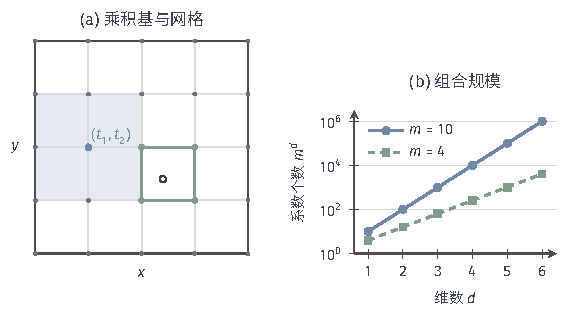
\includegraphics[width=95.0mm]{figures/02-abstract-mathematics/03-function-spaces/tikz/c6-tensor-grid/figure.pdf}
  \caption{张量积网格。(a)~每轴$m=5$个结点，蓝底为乘积帽形基$\varphi_1(x)\varphi_2(y)$的支撑，蓝点为其中心结点$(t_1,t_2)$；空心圆为一个查询点，双线性插值只用它所在单元的四个角点（绿）。(b)~完整张量积系数个数$m^d$随维数$d$指数增长（对数纵轴）。}
  \label{fig:apx-tensor-grid}
\end{figure}

乘积结构也出现在核方法中。第~\ref{sec:rkhs-kernel-operations}节说明两个核的乘积仍是核；$\mathbb R^d$上的高斯核正是$d$个一维高斯核的乘积，其核截面$K_{(x',y')}=K_{1,x'}\otimes K_{2,y'}$是一维核截面的张量积。插值核的频率性质、混叠和实际重建算法属于前面提到的信号问题，这里不展开。

\subsection{低秩分离表示}
\label{sec:apx-low-rank}

完整的张量积展开使用全部$mn$个系数。若系数矩阵近似低秩，就可以只用少数几个乘积项。本小节固定两组变量，研究
\[
  F_r(x,y)=\sum_{j=1}^r u_j(x)v_j(y)
\]
能以什么误差逼近给定的二元函数，其中$r$称为项数。

\paragraph{指数函数的Taylor分离}

以$E(x,y)=e^{xy}$、$(x,y)\in[-1,1]^2$为例。把$t=xy$代入指数函数的Taylor展开并截断，
\begin{equation}
  E_r(x,y)=\sum_{k=0}^{r-1}\frac{x^k y^k}{k!},
  \label{eq:apx-exp-taylor}
\end{equation}
每一项都是$x^k/k!$与$y^k$的乘积，所以$E_r$恰有$r$个分离项。由一元Taylor余项，对$|t|\le1$有$|e^t-\sum_{k<r}t^k/k!|\le e^{|t|}|t|^r/r!\le e/r!$，因此
\[
  \|E-E_r\|_\infty\le\frac{e}{r!}.
\]
实际一致误差在$x=y=1$处取得，等于$e-\sum_{k<r}1/k!$；例如$r=4$时为$e-8/3\approx0.0516$，而上界为$e/24\approx0.113$。图~\ref{fig:apx-lowrank-errors}(a)比较了$r=1,\ldots,8$的实际误差与上界。

这个构造证明了存在一个误差至多$e/r!$的$r$项表示，但没有说明它在所有$r$项表示中是否最好。下面会看到，在$L^2$误差下它并不是最好的。

\paragraph{分离秩无限}

既然每个$E_r$都是有限项，自然要问$E$本身是否也能写成有限个乘积之和。答案是否定的，证明依靠指数和的零点计数。

\begin{lemma}[指数和的零点]
\label{lem:apx-exponential-sum-zeros}
设$\lambda_1<\cdots<\lambda_n$为互异实数，实系数$c_1,\ldots,c_n$不全为零。则$g(t)=\sum_{b=1}^nc_be^{\lambda_bt}$在$\mathbb R$上至多有$n-1$个零点。
\end{lemma}

\begin{proof}
对$n$归纳。$n=1$时$g=c_1e^{\lambda_1t}$没有零点。设结论对$n-1$项成立，不妨设$c_n\ne0$（否则项数更少）。$e^{-\lambda_1t}g(t)=c_1+\sum_{b\ge2}c_be^{(\lambda_b-\lambda_1)t}$与$g$零点相同。若它有$n$个零点，由Rolle定理，其导数$\sum_{b\ge2}c_b(\lambda_b-\lambda_1)e^{(\lambda_b-\lambda_1)t}$至少有$n-1$个零点；这是$n-1$项的指数和，系数$c_n(\lambda_n-\lambda_1)\ne0$，与归纳假设矛盾。
\end{proof}

现在设$e^{xy}=\sum_{j=1}^ru_j(x)v_j(y)$对$x,y\in[-1,1]$成立。取互异点$x_1,\ldots,x_{r+1}$与$y_1,\ldots,y_{r+1}$，矩阵$[e^{x_ay_b}]_{a,b}=\sum_j[u_j(x_a)]_a[v_j(y_b)]_b^{\top}$是$r$个秩一矩阵之和，秩至多为$r$，因而存在非零向量$\bm c$使$\sum_bc_be^{x_ay_b}=0$对$a=1,\ldots,r+1$成立。这说明$r+1$项的指数和$\sum_bc_be^{y_bt}$有$r+1$个零点$x_1,\ldots,x_{r+1}$，与引理~\ref{lem:apx-exponential-sum-zeros}矛盾。因此$e^{xy}$不是任何有限个乘积函数之和，只能被逼近，不能被有限项精确表示。

\paragraph{正交基下的最佳低秩截断}

要找最好的$r$项近似，需要先固定误差范数和允许的因子。设$\{e_i\}_{i=1}^m$与$\{f_k\}_{k=1}^n$分别是$L^2(\mu)$与$L^2(\nu)$中的标准正交组，$F=\sum_{i,k}c_{i,k}e_i\otimes f_k$。由定理~\ref{thm:apx-product-basis}前的计算，$\{e_i\otimes f_k\}$标准正交，所以
\[
  \|F\|_{L^2(\mu\otimes\nu)}=\|\bm C\|_F,
\]
即函数的$L^2$范数等于系数矩阵的Frobenius范数。若因子限制在这两个子空间中，$r$项表示$F_r$的系数矩阵秩至多为$r$，误差$\|F-F_r\|=\|\bm C-\bm C_r\|_F$。由Eckart--Young定理\cite{eckart1936}，最优的$\bm C_r$是$\bm C$的截断奇异值分解，最小误差为$\bigl(\sum_{j>r}\sigma_j^2\bigr)^{1/2}$，$\sigma_j$为$\bm C$的奇异值；矩阵的截断奇异值分解及其最优性可参考\BookChapterRef{chap:matrix-analysis}{卷一“谱和奇异值”章}。

允许因子取遍整个$L^2$空间，并不能做得更好。记$P$、$Q$为到两个子空间的正交投影，则$P\otimes Q$把$r$项表示映成至多$r$项的表示，且$F$在它的值域中，于是
\[
  \|F-F_r\|^2=\|F-(P\otimes Q)F_r\|^2+\|(I-P\otimes Q)F_r\|^2\ge\|F-(P\otimes Q)F_r\|^2 .
\]
最优解总可以取在子空间内。

对$e^{xy}$，取$[-1,1]$上标准正交化的Legendre多项式作基（前$14$个，系数由数值求积计算），奇异值依次约为$2.12$、$0.708$、$0.0892$、$0.00763$、$4.84\times10^{-4}$，迅速衰减。图~\ref{fig:apx-lowrank-errors}(b)比较两种$r$项近似的$L^2$误差：$r=4$时Taylor截断为$9.59\times10^{-3}$，最佳秩$4$截断为$4.85\times10^{-4}$，小约二十倍，而且差距随$r$扩大。

\begin{figure}[!htb]
  \centering
  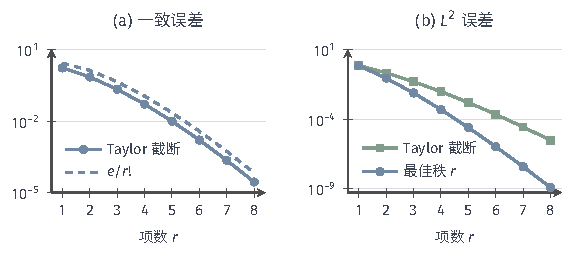
\includegraphics[width=95.9mm]{figures/02-abstract-mathematics/03-function-spaces/tikz/c6-lowrank-errors/figure.pdf}
  \caption{$e^{xy}$在$[-1,1]^2$上的$r$项分离逼近，对数纵轴。(a)~Taylor截断$E_r$的一致误差（实线）与上界$e/r!$（虚线）。(b)~$L^2$误差：Taylor截断（方块）与最佳秩$r$截断（圆点），后者由Legendre正交基下系数矩阵的奇异值算出，为$(\sum_{j>r}\sigma_j^2)^{1/2}$。可行的构造不一定最优。}
  \label{fig:apx-lowrank-errors}
\end{figure}

\paragraph{非正交基与Gram矩阵}

上面的结论依赖基的正交性。若$\bm\varphi$、$\bm\psi$不正交，记Gram矩阵$\bm G_\varphi=[\langle\varphi_i,\varphi_{i'}\rangle]$、$\bm G_\psi=[\langle\psi_k,\psi_{k'}\rangle]$，由式~\eqref{eq:apx-coefficient-matrix}和式~\eqref{eq:apx-product-inner}，
\[
  \|F\|^2=\int\!\!\int\bm\varphi^{\top}\bm C\bm\psi\bm\psi^{\top}\bm C^{\top}\bm\varphi\,\mathrm d\mu\,\mathrm d\nu
  =\operatorname{tr}\bigl(\bm C\bm G_\psi\bm C^{\top}\bm G_\varphi\bigr)
  =\bigl\|\bm G_\varphi^{1/2}\bm C\bm G_\psi^{1/2}\bigr\|_F^2 .
\]
因此最佳截断应作用于加权矩阵$\bm G_\varphi^{1/2}\bm C\bm G_\psi^{1/2}$，截断后再变换回原系数；直接截断$\bm C$的奇异值分解，一般不是$L^2$最优的。

$e^{xy}$恰好是一个例子。在单项式基$\{1,x,x^2,\ldots\}$下，Taylor系数矩阵是对角阵$\operatorname{diag}(1,1,1/2!,1/3!,\ldots)$，它的截断奇异值分解正是Taylor截断$E_r$。单项式基不正交，所以这个截断不是最佳的，图~\ref{fig:apx-lowrank-errors}(b)中两条曲线的差距就来自这里。

\paragraph{项数、因子幅度与高阶情形}

项数$r$、因子的幅度和误差是三个不同的量。同一个乘积可以写成$u\otimes v=(\lambda u)\otimes(v/\lambda)$，因子的大小不由函数决定；两项之差$M\,u\otimes v-M\,u\otimes v'$在$v'$接近$v$时可以很小，而每个因子的范数都含有$M$。只给出项数，既不能控制输出的大小，也不能保证计算稳定。

两组变量的结论依赖矩阵的奇异值分解，不能直接推广到三组及以上的变量。考虑三元函数$T(x,y,z)=x+y+z$，令
\[
  T_n(x,y,z)=n\Bigl(1+\frac xn\Bigr)\Bigl(1+\frac yn\Bigr)\Bigl(1+\frac zn\Bigr)-n .
\]
展开得$T_n=T+(xy+yz+zx)/n+xyz/n^2$，在有界区域上一致收敛到$T$，而每个$T_n$只有两个乘积项（常数$-n$也是乘积函数）。另一方面，$T$不能写成两个三元乘积之和：把任一表示投影到每个变量的$\operatorname{span}\{1,x\}$上，问题化为$2\times2\times2$张量的秩，而对应张量的秩为$3$\scite{desilva2008tensor}。于是$T$到两项表示的距离为零却无法达到，最佳两项近似不存在；逼近列$T_n$的因子幅度还随$n$发散。高阶情形的低秩逼近需要专门的理论，不能套用矩阵截断公式。
